\documentclass{standalone}
\usepackage{tikz}
\begin{document}
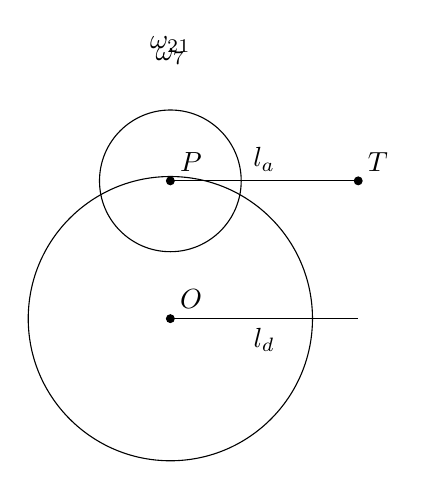
\begin{tikzpicture}[scale=0.7]
  \filldraw (0.0, 0.0) circle (2pt) node[above right] {$P$};
  \filldraw (3.4083, 0.0) circle (2pt) node[above right] {$T$};
  \filldraw (0.0, -2.5) circle (2pt) node[above right] {$O$};
  \draw (0.0, 0.0) -- (3.4083, 0.0) node[midway, above] {$l_a$};
  \draw (0.0, -2.5) -- (3.4083, -2.5) node[midway, below] {$l_d$};
  \draw (0.0, 0.0) circle (1.2855) node[above=1.5cm] {$\omega_{21}$};
  \draw (0.0, -2.5) circle (2.5786) node[above=3.1cm] {$\omega_7$};
\end{tikzpicture}
\end{document}